\documentclass[12pt,a4paper]{article}
\usepackage[utf8]{inputenc}
\usepackage[T1]{fontenc}
\usepackage{lmodern}
\usepackage{geometry}
\geometry{margin=2.5cm}
\usepackage{booktabs}
\usepackage{longtable}
\usepackage{array}
\usepackage{hyperref}
\usepackage{float}
\usepackage{graphicx}

\title{Homework 3: RAG for Science Question Answering}
\author{RNN and Transformer Course}
\date{Spring 2026}

\begin{document}
\maketitle

\begin{abstract}
This report presents the official Homework 3 pipeline using a 50-question random sample from the specified Kaggle \texttt{train.csv} file with \texttt{random\_state=42}. The system compares two chunking strategies, builds two FAISS indices with \texttt{BAAI/bge-m3}, applies two-stage retrieval with dense search followed by \texttt{cross-encoder/ms-marco-MiniLM-L-6-v2}, and generates final answers with local Ollama \texttt{llama3}. On the official evaluation set, the final generation pipeline reached \textbf{70.00\% accuracy (35/50)}. A previous science-only / DeepSeek / ensemble branch is retained only as an optional appendix and is not used as the formal HW3 score.
\end{abstract}

\tableofcontents
\newpage

\section{Introduction}

The goal of Homework 3 is to build a retrieval-augmented generation pipeline for science question answering. The official submission in this report follows the required structure:

\begin{itemize}
    \item Part 1: compare two chunking strategies and build two vector indices.
    \item Part 2: implement dense retrieval plus cross-encoder re-ranking and compare hit rate.
    \item Part 3: use Ollama Llama-3 to answer multiple-choice questions from retrieved evidence.
    \item Latency analysis: measure vector search, re-ranking, and generation time on the same official pipeline.
\end{itemize}

\section{Dataset and Official Evaluation Setup}

\subsection{Random 50-question sample from train.csv}

The official evaluation set is created directly from the specified Kaggle train file:

\begin{verbatim}
train\_path = r"D:\\course\\rnnlstm\\HW3\\kaggle-llm-science-exam\\train.csv"
train\_df = pd.read\_csv(train\_path)
official\_eval\_df = train\_df.sample(n=50, random\_state=42).reset\_index(drop=True)
official\_eval\_df = official\_eval\_df.rename(columns={"prompt": "question"})
\end{verbatim}

This produces a fixed 50-question sample from the 200 training rows in the specified file. This is the only dataset used for the formal HW3 results in this report.

\subsection{Wikipedia corpus construction}

The cached \texttt{official\_wiki\_articles.json} is used as the local Wikipedia plain-text corpus for this assignment run. Articles are converted into document objects before chunking.

\begin{table}[H]
\centering
\begin{tabular}{lr}
\toprule
\textbf{Metric} & \textbf{Value} \\
\midrule
specified \texttt{train.csv} rows & 200 \\
Official evaluation rows & 50 \\
Raw Wikipedia documents & 500 \\
Total raw corpus characters & 2,252,107 \\
\bottomrule
\end{tabular}
\end{table}

\section{Part 1: Indexing Pipeline}

\subsection{Chunking Strategy A}

Strategy A uses fixed-size recursive chunking with \texttt{chunk\_size=500} and \texttt{overlap=50}. This is the smaller-granularity baseline index.

\subsection{Chunking Strategy B}

Strategy B uses larger recursive chunks with \texttt{chunk\_size=1000} and \texttt{overlap=200}. This keeps more local context inside each chunk.

\subsection{Vector Index Construction}

Both indices use the same embedding model and GPU execution:

\begin{itemize}
    \item Embedding model: \texttt{BAAI/bge-m3}
    \item Vector store: FAISS
    \item Device: CUDA GPU
\end{itemize}

Index A stores Strategy A chunks, and Index B stores Strategy B chunks.

\subsection{Chunk Size Analysis}

\begin{table}[H]
\centering
\begin{tabular}{lrr}
\toprule
\textbf{Metric} & \textbf{Strategy A} & \textbf{Strategy B} \\
\midrule
Chunk size & 500 & 1000 \\
Overlap & 50 & 200 \\
Number of chunks & 6,865 & 3,204 \\
Average chunk length (chars) & 334.48 & 732.73 \\
Maximum chunk length (chars) & 500 & 1000 \\
\bottomrule
\end{tabular}
\end{table}

Strategy A creates many shorter chunks, while Strategy B produces fewer but longer chunks. In this rerun, smaller chunks more frequently cut sentence boundaries and split complete answer spans across chunk edges, while Strategy B preserved longer contiguous evidence and gave more reliable complete-answer capture.

\begin{figure}[H]
\centering
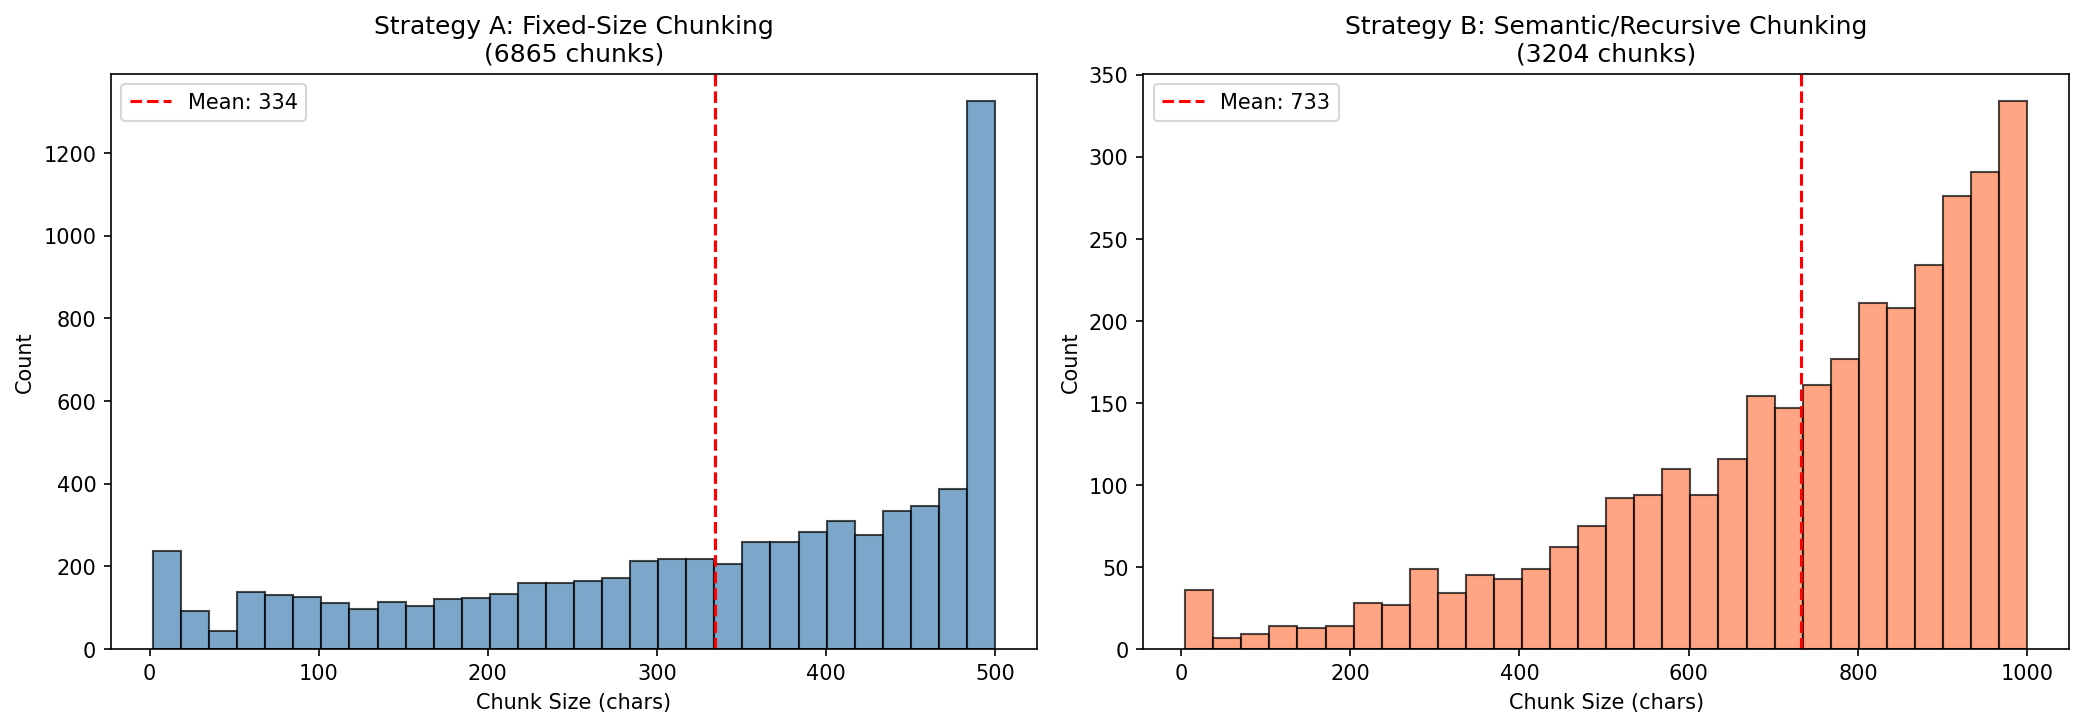
\includegraphics[width=0.78\textwidth]{chunk_size_distribution.png}
\caption{Chunk-size distribution from the notebook run.}
\end{figure}

\section{Part 2: Retrieval and Re-ranking}

\subsection{Dense Retrieval}

Stage 1 retrieval uses dense vector search over each FAISS index with \texttt{top\_k=20}.

\subsection{Cross-Encoder Re-ranking}

Stage 2 uses \texttt{cross-encoder/ms-marco-MiniLM-L-6-v2} to score the 20 retrieved candidates and keep the top 3 chunks for generation.

\subsection{Hit Rate Comparison}

Hit rate is reported as a retrieval proxy metric based on keyword overlap between the retrieved chunks and the correct answer text. The assignment requires this comparison, so it is kept explicitly as a proxy retrieval metric rather than a perfect relevance label.

\begin{table}[H]
\centering
\begin{tabular}{p{6.0cm}p{5.5cm}r}
\toprule
\textbf{Index} & \textbf{Method} & \textbf{Hit Rate} \\
\midrule
Index A (fixed 500/50) & Vector Search Only & 66.00\% \\
Index A (fixed 500/50) & Vector Search + Re-ranking & 72.00\% \\
Index B (recursive 1000/200) & Vector Search Only & 78.00\% \\
Index B (recursive 1000/200) & Vector Search + Re-ranking & 78.00\% \\
\bottomrule
\end{tabular}
\end{table}

On this official 50-question sample, Strategy B gives the strongest vector-only hit-rate proxy, while the final official generation pipeline uses Strategy B with re-ranking as the required two-stage retrieval setup. Re-ranking improves Index A and ties Index B on this proxy table; therefore we report gains carefully as retrieval-proxy improvements and still rely on end-to-end QA accuracy for final assessment.

\begin{figure}[H]
\centering
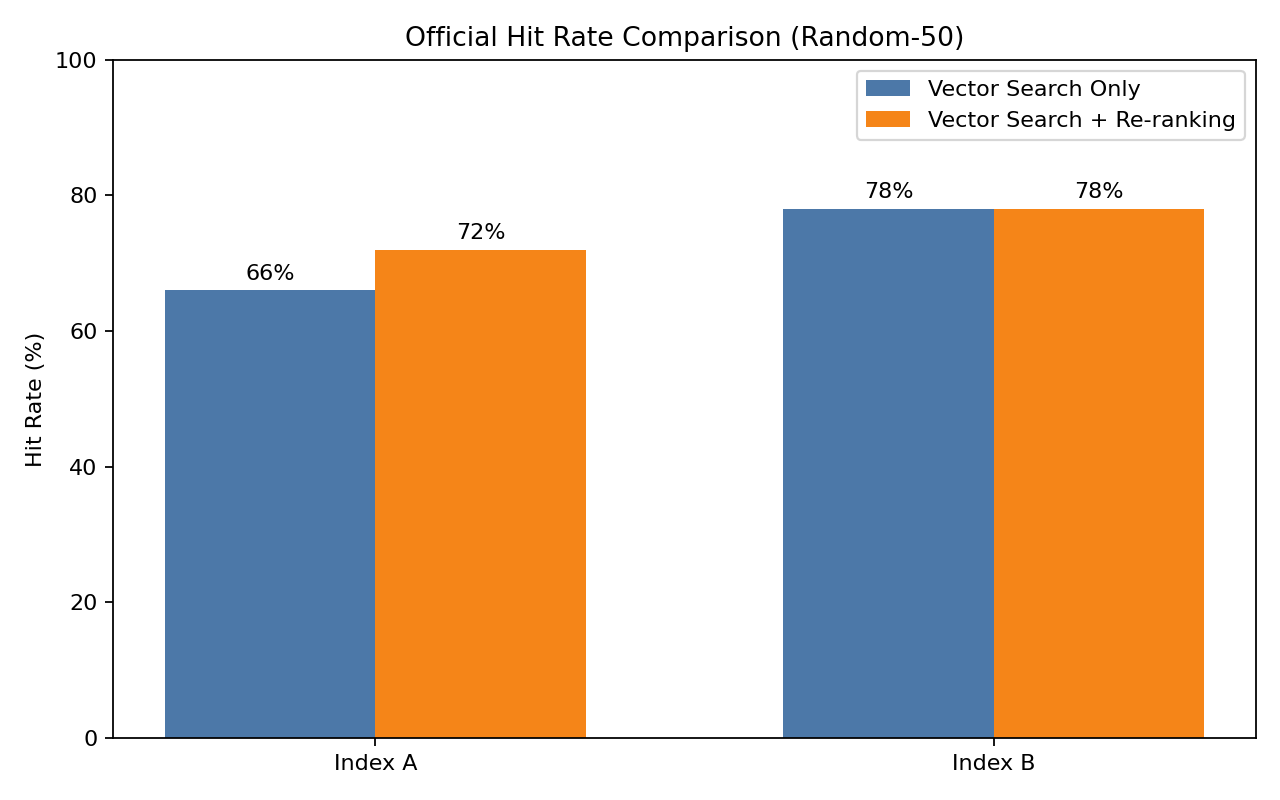
\includegraphics[width=0.72\textwidth]{hit_rate_comparison.png}
\caption{Official hit-rate comparison from the notebook run.}
\end{figure}

\subsection{Two Qualitative Re-ranking Examples}

The following two cases were selected from the official random-50 evaluation set. They show cases where vector search ranked a weak or irrelevant chunk first, while cross-encoder re-ranking promoted a more answer-relevant chunk to rank 1.

\textbf{Case 1: MOND concept promotion}

\begin{itemize}
    \item Source: official random-50
    \item Question: What is Modified Newtonian Dynamics (MOND)?
    \item Correct answer: \texttt{C. MOND is a hypothesis that proposes a modification of Newton's law of universal gravitation ...}
    \item Vector Search top-1:
    \item snippet: \texttt{Magnetic field}
    \item score: \texttt{-10.3605}
    \item why it is weak / irrelevant: the vector top-1 chunk is off-topic and does not explain MOND or modified gravity.
    \item Re-ranked top-1:
    \item snippet: \texttt{Sir Isaac Newton's laws of motion contain an important formula ... one newton ... acceleration due to earth's gravity ...}
    \item original vector rank: \texttt{6}
    \item score: \texttt{-6.9466}
    \item evidence phrase: \texttt{Newton law of universal gravitation}
    \item why it is more answer-relevant / supports the correct answer: the promoted chunk brings in Newton-law gravity concepts, which are the core concept needed to interpret MOND as a modification framework.
    \item Explanation: cross-encoder re-ranking moved an irrelevant top-1 chunk down and promoted a gravity-concept chunk to rank 1 with a clear score gain.
\end{itemize}

\textbf{Case 2: Light-ion fusion concept promotion}

\begin{itemize}
    \item Source: official random-50
    \item Question: What is accelerator-based light-ion fusion?
    \item Correct answer: \texttt{A. Accelerator-based light-ion fusion is a technique that uses particle accelerators ... to induce light-ion fusion reactions ...}
    \item Vector Search top-1:
    \item snippet: \texttt{Photon interactions with matter}
    \item score: \texttt{-9.7298}
    \item why it is weak / irrelevant: the vector top-1 chunk is about generic photon interactions and does not explain accelerator-based fusion setup.
    \item Re-ranked top-1:
    \item snippet: \texttt{The light and heat created by nuclear fusion makes stars like the Sun very hot ... Fusion makes a lot of energy ...}
    \item original vector rank: \texttt{9}
    \item score: \texttt{-5.8277}
    \item evidence phrase: \texttt{light and heat created by nuclear fusion}
    \item why it is more answer-relevant / supports the correct answer: the promoted chunk directly discusses fusion-process evidence, which is far closer to the correct option than the vector top-1 chunk.
    \item Explanation: cross-encoder re-ranking promoted a fusion-bearing chunk from rank 9 to rank 1 and improved the relevance score.
\end{itemize}

These examples are qualitative evidence-ordering demonstrations and do not change the official random-50 accuracy computation.

\section{Part 3: Ollama Generation}

\subsection{Llama-3 Integration}

The official generator is local Ollama \texttt{llama3}.

\subsection{Anti-hallucination Prompt}

The system prompt enforces two constraints:

\begin{itemize}
    \item use only the retrieved context,
    \item output exactly one letter from \texttt{A/B/C/D/E}.
\end{itemize}

For open-ended RAG usage, the same policy maps insufficient evidence to ``I do not know'', while this HW3 MCQ run enforces single-letter output.

The generator receives the reranked top-3 chunks together with the question and answer choices.

\subsection{Accuracy on 50 Random train.csv Questions}

The official generation pipeline is:

\begin{itemize}
    \item Index B
    \item dense retrieval \texttt{top\_k=20}
    \item cross-encoder re-ranking to top-3
    \item Ollama \texttt{llama3}
\end{itemize}

\begin{table}[H]
\centering
\begin{tabular}{lr}
\toprule
\textbf{Metric} & \textbf{Value} \\
\midrule
Official accuracy & 70.00\% \\
Correct answers & 35 / 50 \\
\bottomrule
\end{tabular}
\end{table}

This is the formal HW3 score reported in the notebook and report.

\section{Latency Analysis}

Latency is measured on the same official pipeline and evaluation set.

\begin{table}[H]
\centering
\begin{tabular}{lr}
\toprule
\textbf{Stage} & \textbf{Average Latency (s)} \\
\midrule
Vector search & 0.0123 \\
Re-ranking & 0.0156 \\
LLM generation & 2.3950 \\
Total & 2.4229 \\
\bottomrule
\end{tabular}
\end{table}

Re-ranking adds about 15.6 milliseconds on average, which is very small compared with the 2.395-second LLM generation stage. On this rerun, proxy hit rate improves on Index A and ties on Index B, so re-ranking remains a low-cost stage that is operationally worthwhile in this pipeline.

\begin{figure}[H]
\centering
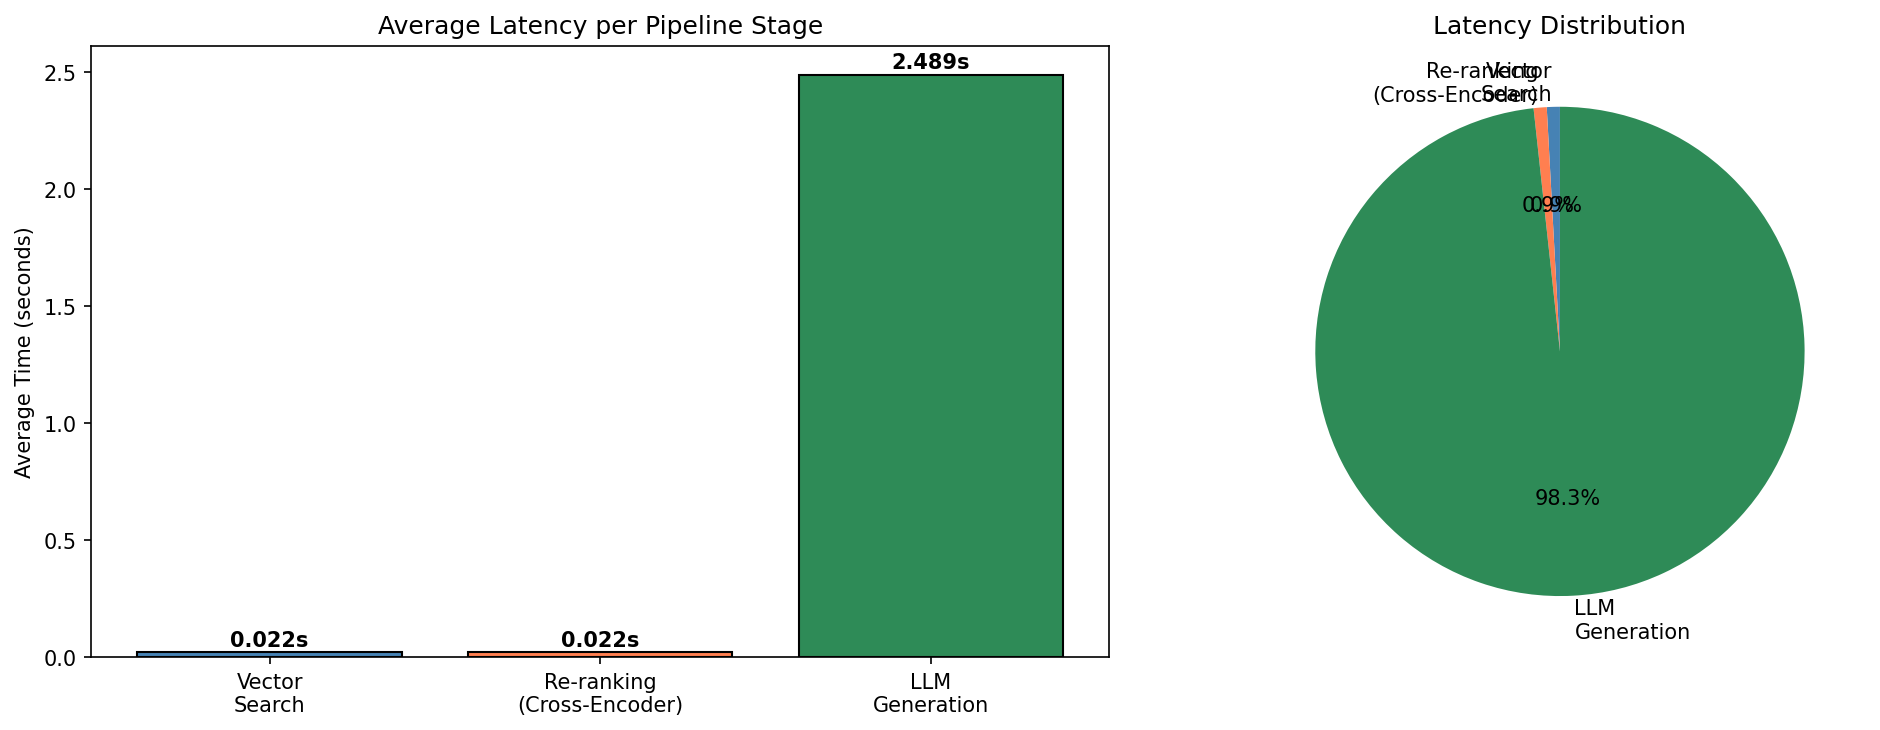
\includegraphics[width=0.72\textwidth]{latency_analysis.png}
\caption{Latency breakdown from the official notebook run.}
\end{figure}

\section{Optional Advanced Experiment}

\subsection{Motivation}

The official random 50-question \texttt{train.csv} sample remains the required HW3 setting. The appendix branch was tested only to study whether stronger retrieval, answer-aware evidence scoring, and model variants improve science-only QA.

\subsection{Science-only evaluation setup}

The advanced branch filtered the public mirror with science keywords, creating a science-only pool with the following traceable setup from \texttt{advanced\_experiment\_summary.json}:

\begin{table}[H]
\centering
\begin{tabular}{lr}
\toprule
\textbf{Metric} & \textbf{Value} \\
\midrule
Public mirror rows & 6,684 \\
Science-only pool rows & 1,469 \\
Science dev rows & 10 \\
Science held-out test rows & 50 \\
\bottomrule
\end{tabular}
\end{table}

This appendix-only setup is not the official HW3 evaluation because it does not use the required random 50-question \texttt{train.csv} sample.

\subsection{Advanced retrieval changes}

The advanced notebook branch (\texttt{hw3advance.ipynb}) implemented:

\begin{itemize}
    \item query rewriting for Wikipedia retrieval,
    \item long-form Wikipedia evidence extraction,
    \item chunk-level re-ranking over fetched evidence,
    \item option-aware evidence scoring,
    \item NLI-style scoring with a DeBERTa entailment model.
\end{itemize}

\subsection{Model and ensemble comparison}

The following advanced appendix numbers are traceable from \texttt{advanced\_experiment\_summary.json} and \texttt{advanced\_rag\_results.csv}:

\begin{table}[H]
\centering
\begin{tabular}{p{9cm}r}
\toprule
\textbf{Appendix experiment} & \textbf{Accuracy} \\
\midrule
Llama 3 model-only on corrected science dev slice & 30.00\% \\
DeepSeek model-only on corrected science dev slice & 40.00\% \\
DeepSeek RAG vector-only & 30.00\% \\
DeepSeek RAG with re-ranking & 60.00\% \\
Option-aware rerank + NLI & 60.00\% \\
Final ensemble on 10-question dev slice & 80.00\% \\
Final ensemble on held-out 50 science-only questions & 72.00\% \\
Post-hoc best rule on the same science-only run & 74.00\% \\
\bottomrule
\end{tabular}
\end{table}

\begin{figure}[H]
\centering
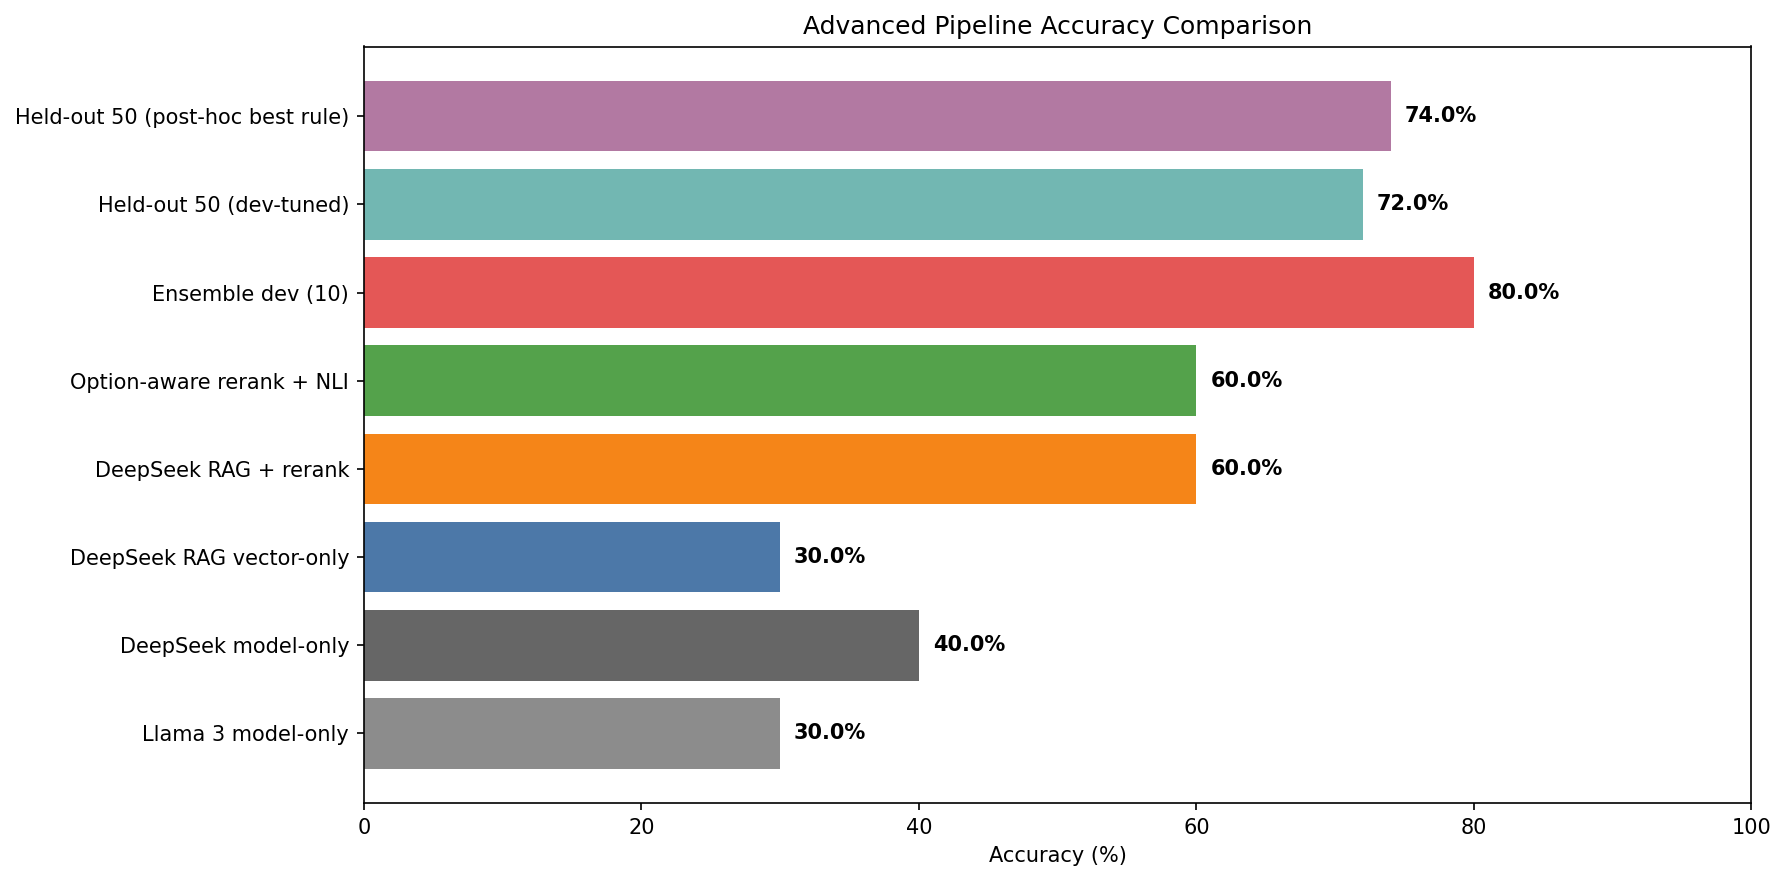
\includegraphics[width=0.72\textwidth]{advanced_accuracy_comparison.png}
\caption{Appendix-only advanced method comparison from notebook outputs.}
\end{figure}

\subsection{Why this is not the official HW3 score}

These results are useful as an ablation and extension appendix, but they are not reported as the formal HW3 score because:

\begin{itemize}
    \item they use a filtered science-only pool rather than the required random 50-question \texttt{train.csv} sample,
    \item they use DeepSeek and ensemble extensions beyond the official Ollama \texttt{llama3} pipeline,
    \item the formal HW3 result in this report remains the official \textbf{70.00\%} score on the random-\texttt{train.csv} evaluation.
\end{itemize}

\section{Conclusion}

The final official HW3 pipeline uses a random 50-question sample from the specified Kaggle \texttt{train.csv} path, two chunking strategies, FAISS retrieval, cross-encoder re-ranking, and Ollama \texttt{llama3} generation on GPU. The final official accuracy is \textbf{70.00\% (35/50)}. Strategy B gives the strongest vector-only hit-rate proxy, while the final official generation pipeline uses Strategy B with re-ranking as the required two-stage retrieval setup. The appendix shows that a science-only DeepSeek/ensemble branch can reach a higher ceiling, but the formal HW3 score reported here remains 70.00\%.

\end{document}
